\documentclass{article}

\usepackage{graphicx}
\usepackage{amsmath}
\usepackage[colorlinks,bookmarks,bookmarksnumbered,allcolors=blue]{hyperref}
\usepackage[capitalise]{cleveref}

\begin{document}

\author{Andrew Ning}
\title{Leapfrogging Vortices}
\date{}  %May 10, 2019}
\maketitle

Vortex rings are pretty neat.  Read this \href{https://en.wikipedia.org/wiki/Vortex_ring}{wikipedia article} to get an idea of what they are.  They can propel themselves quite far when moving through a quiescent fluid.  See some fun videos of vortex rings formed by \href{https://www.youtube.com/watch?v=VbV98Z0QP-k}{a volcano}, \href{https://www.youtube.com/watch?v=ks3aQhEohTE}{dolphins}, and  \href{https://www.youtube.com/watch?v=72LWr7BU8Ao}{a plate in a pool}.  They can also be dangerous, for example with helicopters that \href{https://youtu.be/wddpsnvu0PM?t=75}{descend too quickly}.

If you're really careful, and put one vortex ring right behind another you can have leapfrogging vortices!  Check out this video of a \href{https://youtu.be/Yydb9Mqg9TY}{real-life visualization} of the phenomenon, as well as a \href{https://youtu.be/0LP-MgrXtIM}{2D simulation}, and a neat \href{https://www.youtube.com/watch?v=SPBMEXX5xBI}{3D simulation}.

First a little background.  A single vortex produces a velocity field as shown in \cref{fig:vortex}.  It's a lot like the flow field you might see in a bathtub drain on in a hurricane.  A vortex causes the flow to spin around it in the tangential direction as given by:
\begin{equation}
V_\theta = \frac{\Gamma}{2 \pi r}
\end{equation}
The variable $\Gamma$ is the strength of the vortex and is also called the \emph{circulation}.  If we increase $\Gamma$ then the induced velocities increase proportionally.  Notice that the strength of the vortex decreases as $1/r$.  Thus, really close to the vortex the induced velocities are high (indicated by the longer arrows) and as we move further away from the vortex its strength approaches zero.  The vortex does not induce any radial velocity ($V_r = 0$).

\begin{figure}[htb]
\centering
\includegraphics[width=3.0in]{vortex}
\caption{A point vortex (in blue) inducing a velocity field (in black) with the equation describing the velocity field to the right.}
\label{fig:vortex}
\end{figure}


With that basic background we can simulate leapfrogging vortices in 2D.  If you picture a toroidal vortex intersecting a 2D plane you will have two vortices (like the left pair shown in \cref{fig:vortices}).  From our understanding of vortices we can see how it is self-propelling.  Consider the left pair of vortices (e.g., one ring vortex).  The top vortex induces a velocity on the bottom vortex towards the right.  Simultaneously, the top vortex induces a velocity on the top vortex to the right.  Thus, it pushes itself forward.  With two vortices next to each other, things become even more interesting.

\begin{figure}[htb]
\centering
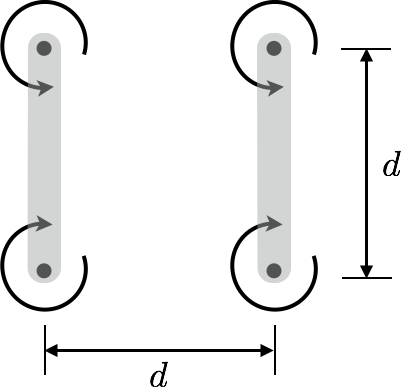
\includegraphics[width=1.5in]{vortices}
\caption{A pair of leapfrogging vortices.}
\label{fig:vortices}
\end{figure}

In this example, make all vortices of equal strength ($\Gamma$).  Each vortex is free to move, and moves with the local fluid velocity.  We will use a basic time stepping method.  Imagine simulating the flight of a ball after it is thrown (we include air resistance so we can't just precompute it using kinematics).  One way to do this is to discretize its motion into small segments of time.  Let's say we have the way to compute the velocity of the ball, if we simulate some small time interval, say a tenth of a second, we could multiply the velocity vector by that time interval and estimate where the ball would have moved at the end of that interval.  We move the ball, recompute the velocity vector, and repeat. This approach is an approximation because the velocity vector really changes continuously and doesn't follow straight lines during time intervals.  However, if we chose a small enough time step the real behavior will be well represented.

Using this procedure you will need to compute the influence of each vortex on every other.  From that induced velocity you can then update the location of all the vortices and repeat.  You need to use a small enough time step to ensure stability.  You may need to try smaller time steps to make sure that your simulation is accurate.

Hint (if you're comfortable with vectors): In vector form, the induced velocity from a vortex is:
\begin{equation}
    \begin{aligned}
        \vec{V} &= \frac{\vec{\Gamma} \times \hat{r}}{2 \pi r}\\
        &= \frac{\vec{\Gamma} \times \vec{r}}{2 \pi r^2}
    \end{aligned}
\end{equation}

\subsubsection*{Deliverables}

\begin{enumerate}
    \item \textbf{Code:} Implement the leapfrogging vortices and plot the resulting trajectories. Make sure your plots are clear and easily understood.  You are welcome to prototype in any programming language you want, but your final submission needs to be in Julia (or Python if requested by your graduated mentor).  Julia is probably a new language for you.  If you're familiar with another language like Matlab you'll be able to pick this up relatively quickly.  However, if programming is new to you this is probably where you will spend most of your time. Judd put together a helpful introduction to Julia \href{https://github.com/byuflowlab/undergrad-onboarding/blob/master/julia.md}{here}.
    
    Use git for version control as you develop the code.  If you are unfamiliar with git, \href{https://guides.github.com/introduction/git-handbook/}{here} is a basic overview.  You won't need to branch or do pull requests when working in your own repo.  You can use a GUI like GitHub Desktop to make this easier, or you can use the command line if comfortable (see bonus below).  Create an account on \href{https://github.com}{GitHub} so that you can create your own repositories.  You'll need to send the link to your repository (with the code) as part of your submission.
    
    \item \textbf{Report:} Write a short scientific report with an introduction, methodology, and results.  See \href{https://me.byu.edu/resources}{BYU ME Writing Materials on the IMRaD genre} for some guidance and examples on scientific writing if this style of writing is new to you.  You will need to use LaTeX.  If you are unfamiliar with LaTeX \href{https://www.overleaf.com/learn/latex/Learn_LaTeX_in_30_minutes}{here} is a 30 minute tutorial.  
\end{enumerate}

\subsubsection*{Bonus (not required)}
\begin{enumerate}
    \item Start learning about the command line.  The command line is the text-based interface to your computer.  You won't need to know anything about the command line to complete this assignment, but it is widely used in the lab and in scientific computing in general.  Step 1 and 2 of \href{https://www.codecademy.com/learn/learn-the-command-line}{this tutorial} would be a good place to start, but feel free to learn more as interested.  For Mac OS or Linux you will use Terminal.  For Windows, the built in command line (DOS) is totally different and not of use to us. Instead you will need to install \href{https://docs.microsoft.com/en-us/windows/wsl/about}{Windows Subsystem for Linux}.  Newer versions of Windows may include it already.
    \item A static image of leapfrogging vortices isn't as fun.  See if you can create an animation so that you can actually watch the movement in time.  You might also like to draw a line between the vortex pairs to better visualize them as a connected ring.
\end{enumerate}


\end{document}